\chapter{Métodos experimentales}

\section{Escritura de guías de onda \label{cap:fs}}
\begin{figure}[H]
	\centering
	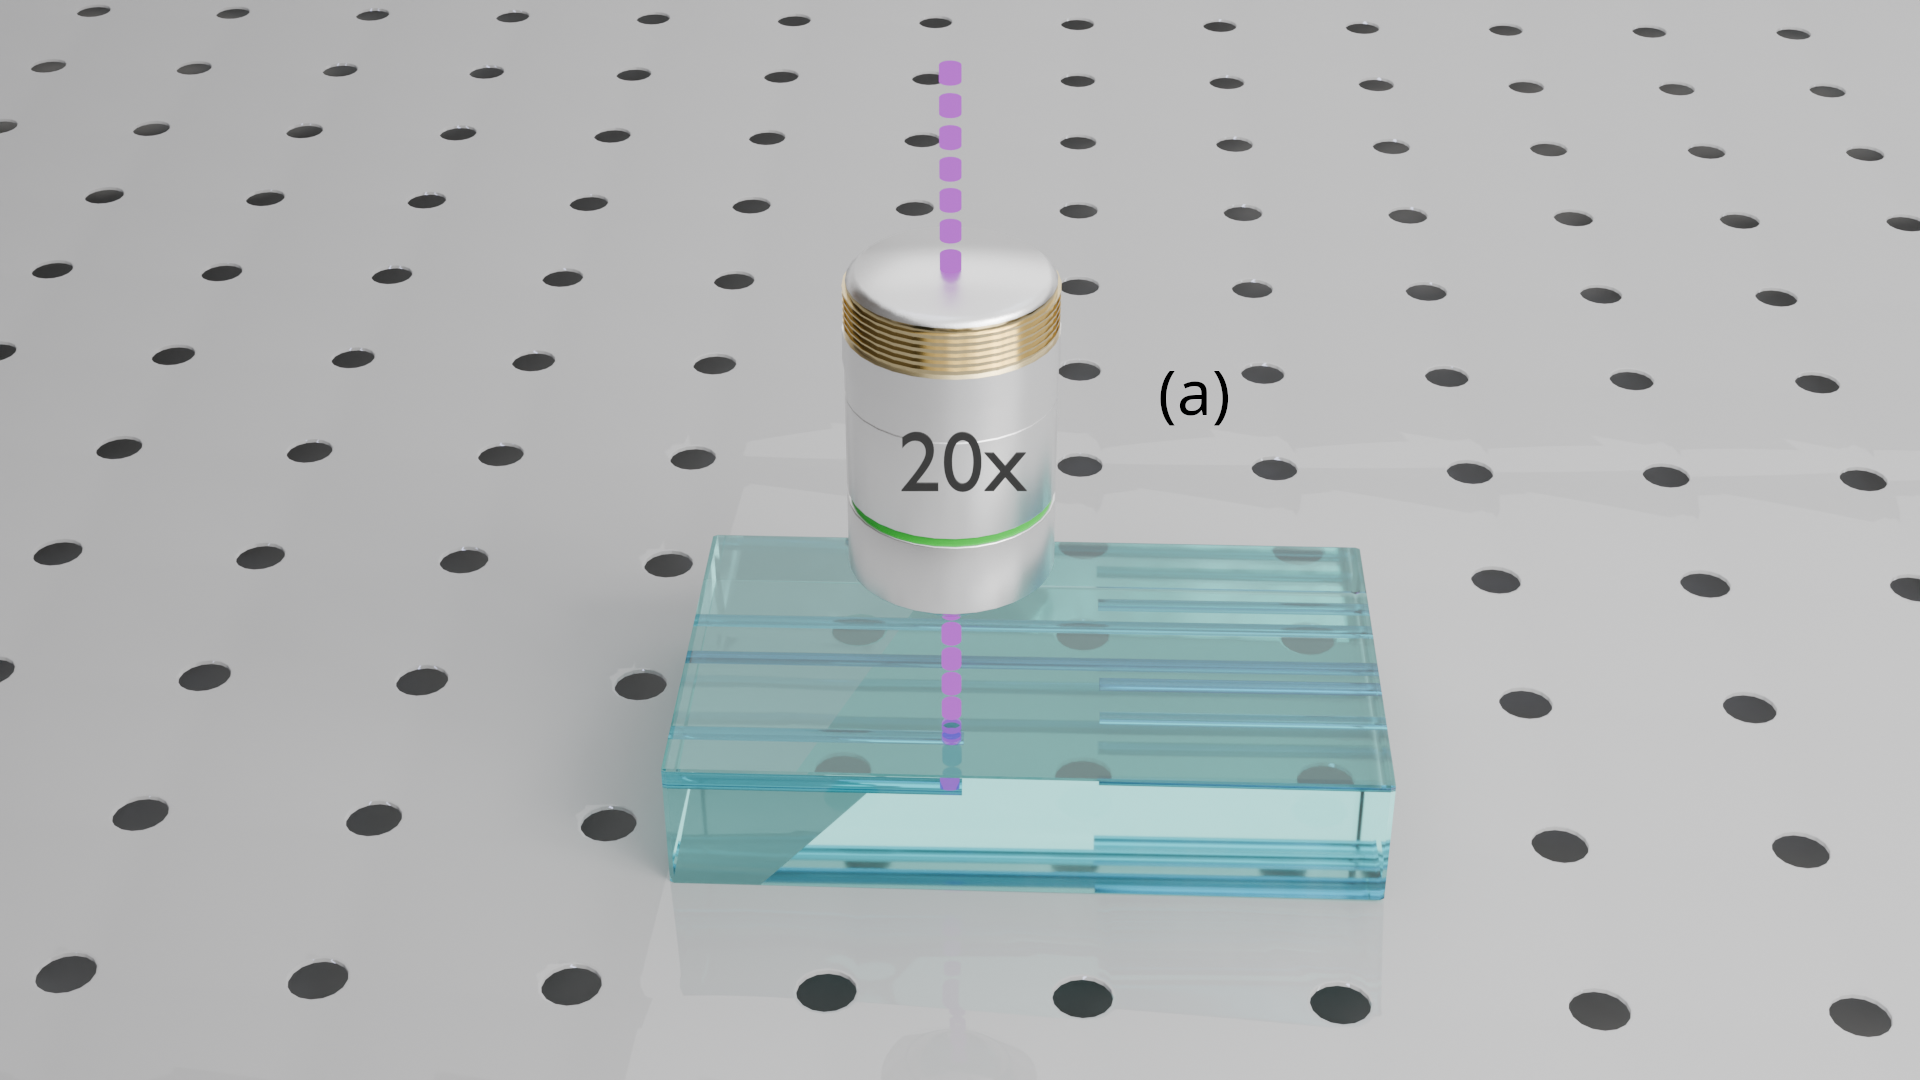
\includegraphics[width=0.6\linewidth, trim={18cm 4cm 15cm 6cm},clip]{media/fabrication}
	\caption{Escritura.}
\end{figure}

\section{Montaje de excitación láser supercontinuo}
\begin{figure}[H]
	\centering
	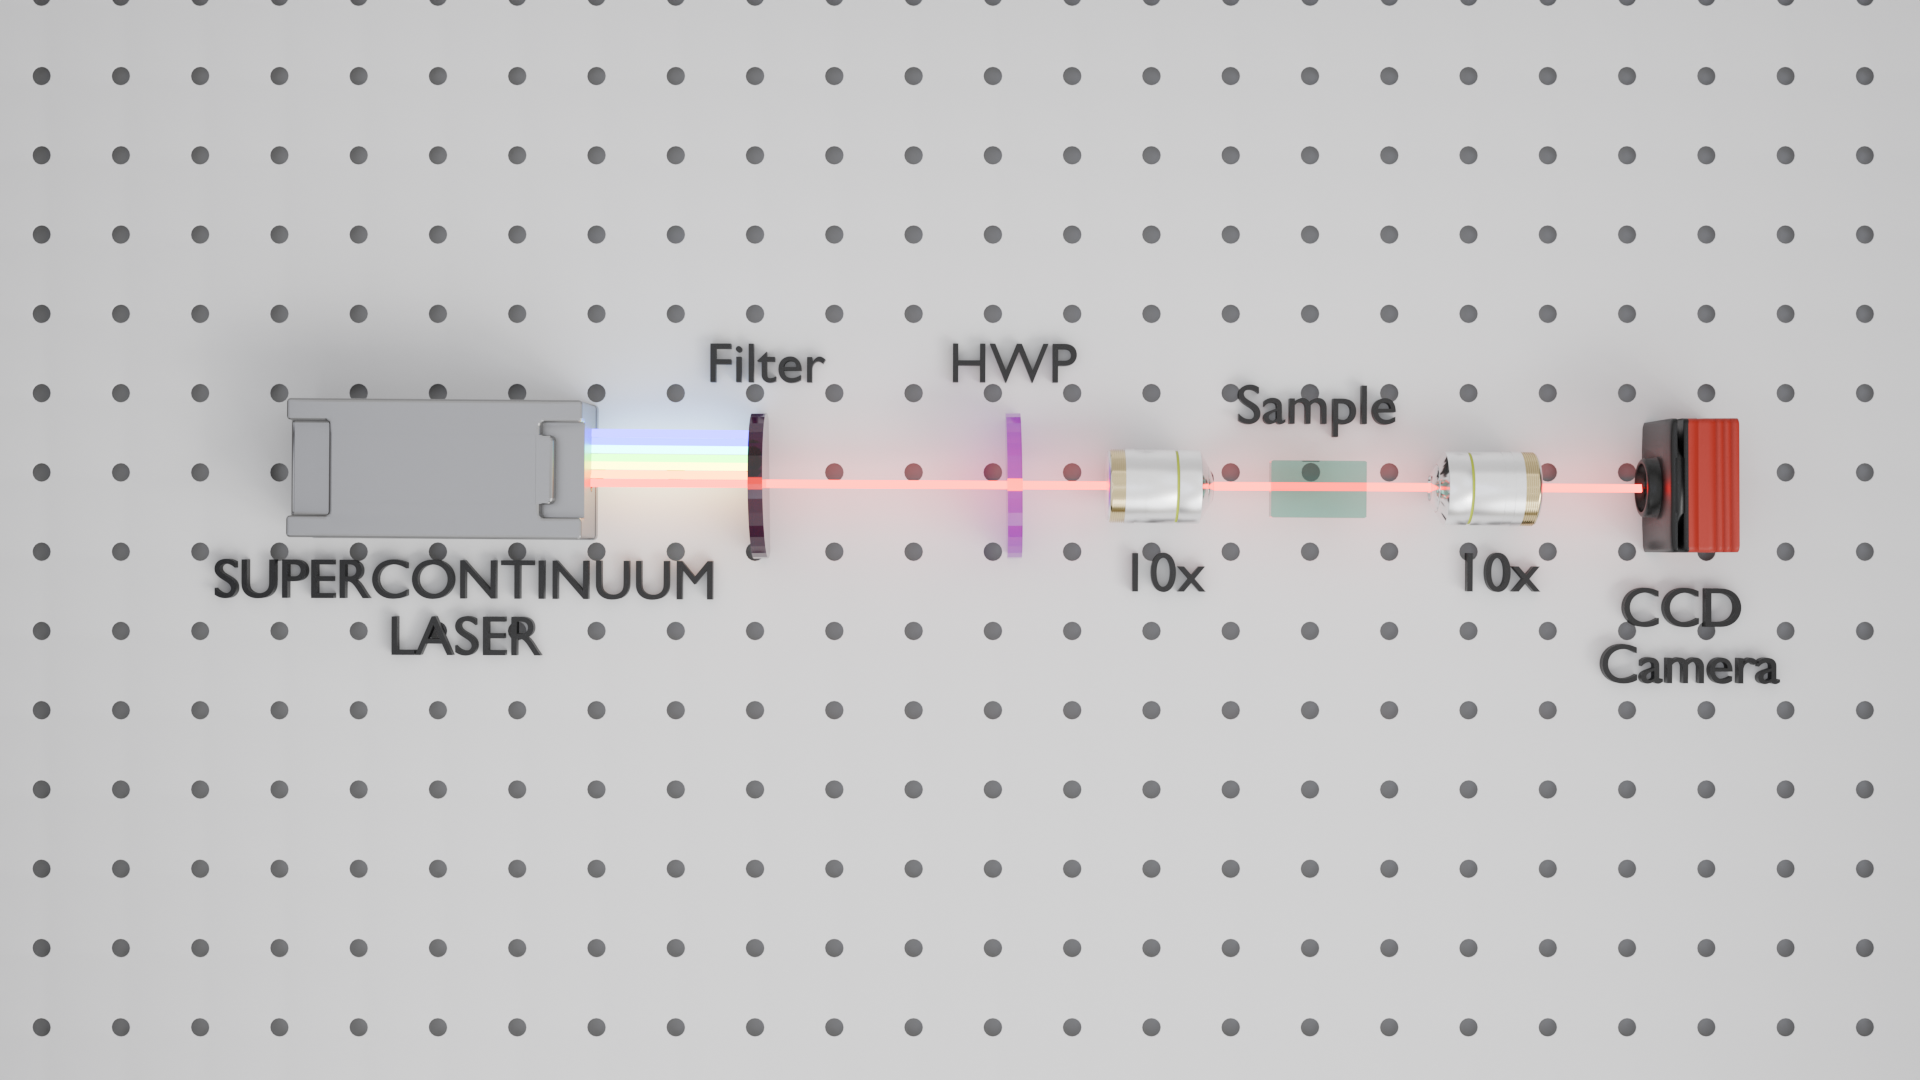
\includegraphics[width=\linewidth, trim={5cm 9cm 3cm 7cm},clip]{media/SC_setup}
	\caption{Montaje SC.}
\end{figure}

\section{Montaje de modulación espacial de luz}

Para usar condiciones iniciales distintas a una gaussiana se hace necesario incorporar métodos de modulación espacial de luz. En esta tesis se utilizó una técnica conocida como 

\subsection{Etapa premodulación}
	El modulador espacial de luz utilizado es un HOLOEYE PLUTO-NIR SLM -  Reflective LCOS, cuya respuesta óptica ocurre con polarización paralela al plano de la mesa óptica. Se utiliza un retardador de media onda ($\lambda/2$) seguido de un polarizador de atenuación 10000:1 con el objetivo de que la polarización de la luz láser coincida con la de la respuesta del SLM. Posteriormente se magnifica y se colima el haz para que abarque todo el área de pixeles disponible con un par de lentes 20x y $L_1$ de foco 100mm. 
\subsection{Etapa de modulación}
	Una rejilla de difracción que maximiza la potencia del primer orden de difracción es utilizada. Para modular en amplitud se debe multiplicar la rejilla por la máscara de amplitud deseada, mientras que para modular en fase basta con sumar el nivel de gris correspondiente a la fase deseada. En la Figura \ref{fig:SLMblaze} se bosqueja el algoritmo implementado en Python en el anexo \ref{sec:codigoSLM}.
	
{
\sidecaptionvpos{figure}{c}
\begin{SCfigure}[]
    \centering
    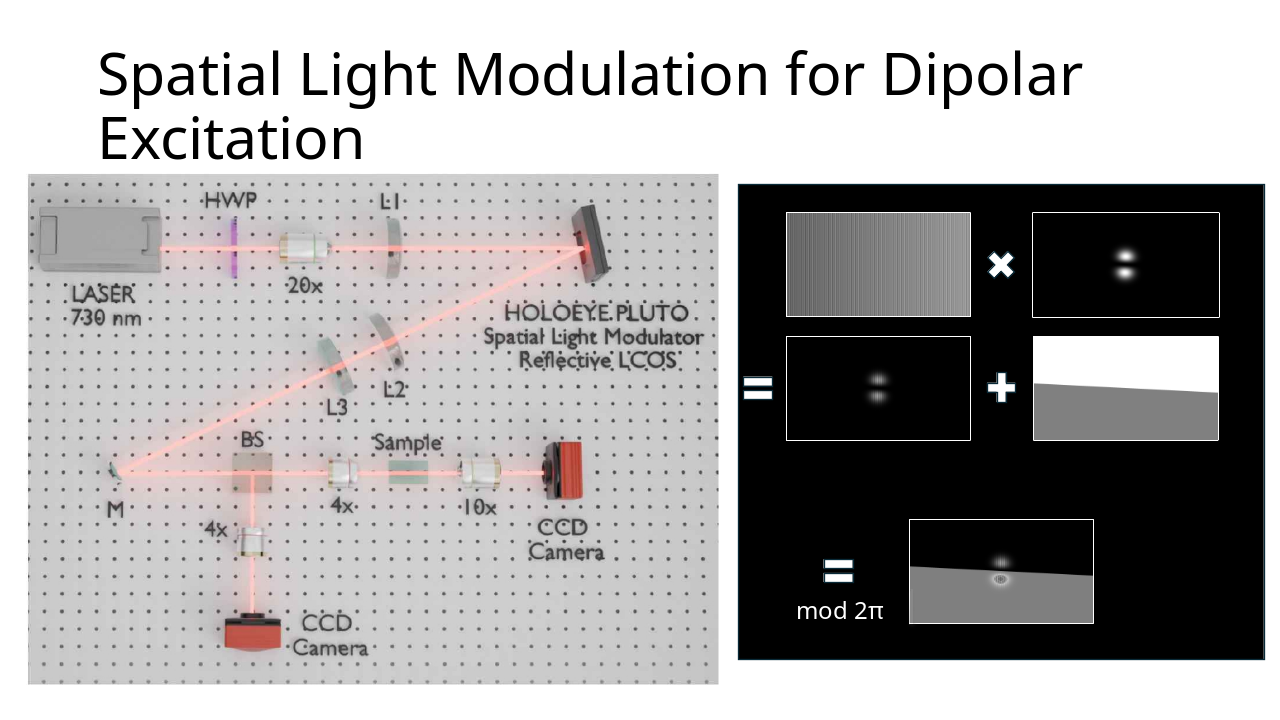
\includegraphics[width=0.35\linewidth, trim={19.5cm 0 0 5cm}, clip]{media/SLMblaze4.png}
    \caption[Algoritmo de modulación espacial de luz para máscaras de amplitud y fase arbitrarias.]{Algoritmo de modulación espacial de luz para máscaras de amplitud y fase arbitrarias. Los parámetros de la rejilla de difracción están sujetos a la longitud de onda usada (730 nm).\label{fig:SLMblaze}}
\end{SCfigure}
}
\subsection{Etapa de acoplamiento}
La imagen modulada pasa por un par de lentes $L_2$ de foco 1000 mm y $L_3$ de foco 50 mm para reducir el tamaño al orden de los micrómetros. La inclinación de la cara de entrada de la muestra debe coincidir con el plano de la imagen modulada, por lo que se generan dos pares de haces gaussianos, unos verticales y otros horizontales, de manera de que al trasladar el lente objetivo 4x, los máximos de difracción se generen en el centro de los haces gaussianos. 
\subsection{Etapa de captura en cámara}
Una vez calibrada la inclinación de la muestra, se fija su posición. Un lente objetivo 10x permite magnificar la imagen de salida y capturar los resultados en un Beam Profiler.
\subsection{Circuito óptico}
\begin{figure}[H]
	\centering
	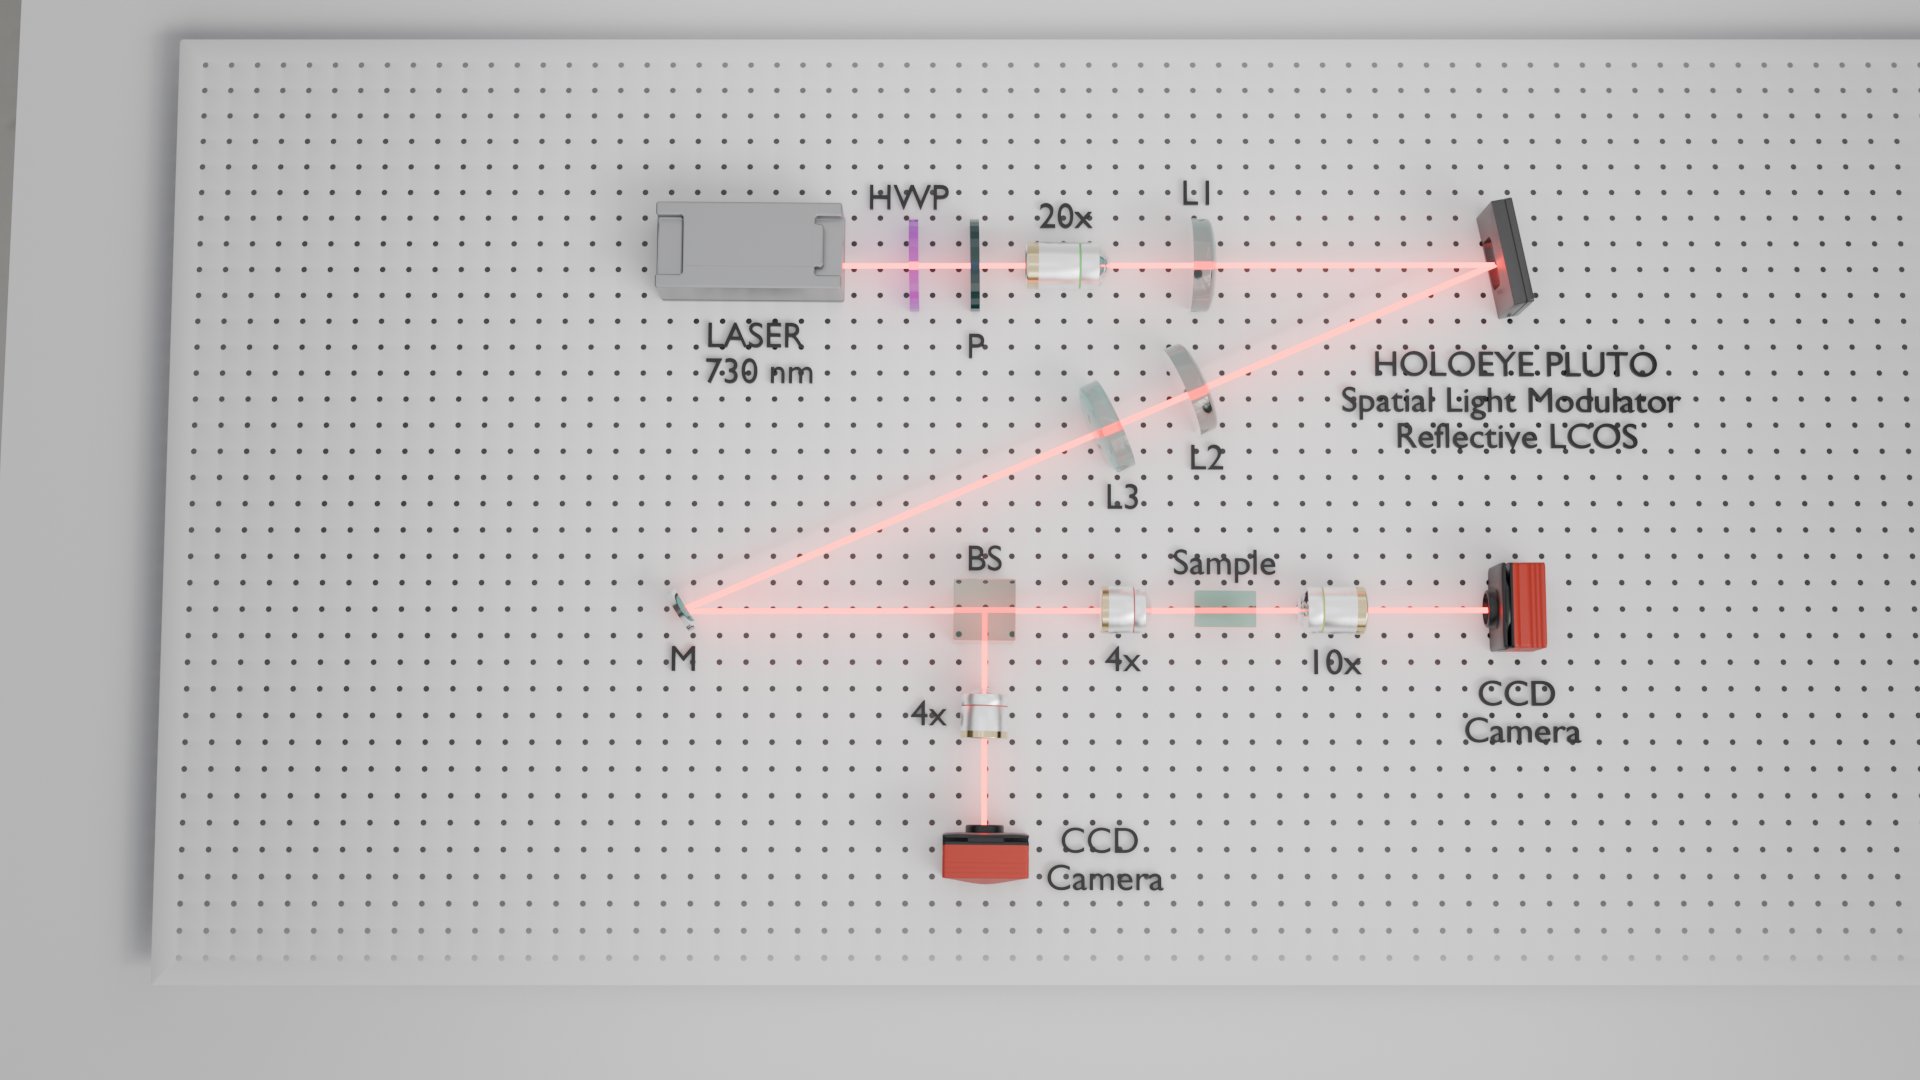
\includegraphics[width=\linewidth, trim={21cm 5cm 7cm 5cm},clip]{media/SLM_setupv1}
\end{figure}

\section{Análisis de imágenes \label{sec:analimag}}
A partir de las imágenes capturadas es posible extraer información de la potencia que contiene cada sitio del sistema fotónico discreto en estudio. Para ello la imagen completa debe ser seccionada equispaciadamente en rectángulos que encierren las regiones donde existen guias de onda, iluminadas o no. La potencia de cada sitio será entonces la suma de la intensidad de cada píxel encerrado en su rectángulo respectivo.

